\documentclass[aspectratio=169]{beamer}

\usepackage[utf8]{inputenc}
\usepackage[english]{babel}
\usepackage{booktabs}
\usepackage{array}
\usepackage{listings}
\usepackage{tikz}
\usetikzlibrary{arrows.meta,positioning,shapes.geometric,calc}

\graphicspath{{logo/}{../logo/}}

\definecolor{ForestGreen}{RGB}{22,100,70}
\definecolor{SoftGreen}{RGB}{229,244,235}
\definecolor{SoftBlue}{RGB}{226,239,255}
\definecolor{SoftOrange}{RGB}{255,241,220}
\definecolor{SoftPurple}{RGB}{239,231,255}

\newcolumntype{L}[1]{>{\raggedright\arraybackslash}p{#1}}

\mode<presentation>{
  \usetheme{Ilmenau}
  \usecolortheme{spruce}
  \usefonttheme{professionalfonts}
  \setbeamertemplate{navigation symbols}{}
  \setbeamertemplate{headline}{}
  \setbeamertemplate{caption}[numbered]
  \setbeamercolor{institute in head/foot}{fg=ForestGreen}
}

\lstdefinestyle{pseudo}{
  language={},
  basicstyle=\ttfamily\scriptsize,
  keywordstyle=\color{blue!75!black}\bfseries,
  morekeywords={FUNCTION,INPUT,OUTPUT,IF,THEN,ELSE,RETURN,FOR,TO,DOWNTO,
    DO,WHILE,REPEAT,UNTIL,MERGE,LEFT,RIGHT,APPEND,LENGTH,SWAP,CREATE,COUNT,PREFIX,COPY,STABLE,MAXIMUM,DIGIT},
  numbers=none,
  showstringspaces=false,
  keepspaces=true,
  columns=fullflexible,
  breaklines=true,
  frame=single,
  rulecolor=\color{ForestGreen!60},
  backgroundcolor=\color{SoftBlue!35},
  tabsize=4
}

% Hide non-positive header line numbers; algorithm steps begin visibly at 1.
\newcommand{\pseudonumberstyle}{%
  \tiny\ifnum\value{lstnumber}>0\color{gray}\else\color{white}\fi}
\lstdefinestyle{pseudonumbered}{
  style=pseudo,
  numbers=left,
  firstnumber=-2,
  numberstyle=\pseudonumberstyle,
  numbersep=6pt,
  numberblanklines=false
}

\tikzset{
  cell/.style={draw=ForestGreen,fill=SoftGreen,thick,minimum width=0.82cm,
    minimum height=0.72cm,align=center},
  active/.style={draw=orange!75!black,fill=SoftOrange,very thick,
    minimum width=0.82cm,minimum height=0.72cm,align=center},
  pivot/.style={draw=purple!70!black,fill=SoftPurple,very thick,
    minimum width=0.82cm,minimum height=0.72cm,align=center},
  process/.style={draw=ForestGreen,rounded corners,fill=SoftGreen,thick,
    minimum height=0.9cm,text width=2.7cm,align=center},
  arrow/.style={-Latex,very thick,ForestGreen}
}

\title[TOKT11105 -- Lecture 4]{Data Structures and Algorithms in Python\\
Lecture 4: Sorting, Selection and Searching Algorithms}
\author{Faculty of Data Science and Artificial Intelligence}
\institute{National Economics University}
\date{}

\AtBeginSection[]{
  \begin{frame}[plain]
    \begin{center}
      \vfill
      {\color{ForestGreen}\large\bfseries SECTION \insertsectionnumber}
      \vspace{0.8em}
      {\color{ForestGreen}\rule{0.68\textwidth}{1.2pt}}
      \vspace{1.1em}
      {\usebeamerfont{section title}\color{ForestGreen}\LARGE\bfseries
        \parbox{0.86\textwidth}{\centering\insertsectionhead\par}}
      \vspace{1.1em}
      {\color{ForestGreen}\rule{0.68\textwidth}{1.2pt}}
      \vfill
    \end{center}
  \end{frame}
}

\begin{document}

\begin{frame}[plain]
  \setbeamercolor{block body example}{bg=ForestGreen,fg=white}
  \begin{center}
    \begin{beamercolorbox}[wd=\textwidth,sep=1pt,center,rounded=true,shadow=true]{block body example}
      \IfFileExists{logo_slide.png}{\includegraphics[width=0.27\textwidth]{logo_slide.png}}{\fcolorbox{ForestGreen}{ForestGreen}{\parbox[c][0.85cm][c]{0.27\textwidth}{\centering\color{white}\bfseries NEU -- DS\&AI}}}
    \end{beamercolorbox}
  \end{center}
  \vspace{-0.25em}
  \titlepage
\end{frame}

\logo{\IfFileExists{logo_fda.png}{\includegraphics[width=0.8cm]{logo_fda.png}}{\fcolorbox{ForestGreen}{ForestGreen}{\parbox[c][0.45cm][c]{0.8cm}{\centering\color{white}\scriptsize FDA}}}}
\setbeamercolor{footline upper}{bg=ForestGreen!22,fg=ForestGreen!85!black}
\setbeamercolor{footline lower}{bg=ForestGreen,fg=white}
\setbeamertemplate{footline}{%
  \leavevmode
  \hbox{%
    \begin{beamercolorbox}[wd=.50\paperwidth,ht=2.35ex,dp=.75ex,
      leftskip=1em]{footline upper}
      Faculty of Data Science and Artificial Intelligence
    \end{beamercolorbox}%
    \begin{beamercolorbox}[wd=.50\paperwidth,ht=2.35ex,dp=.75ex,
      rightskip=1em plus1fil]{footline upper}
      \hfill National Economics University
    \end{beamercolorbox}%
  }
  \hbox{%
    \begin{beamercolorbox}[wd=.72\paperwidth,ht=2.35ex,dp=.75ex,
      leftskip=1em]{footline lower}
      \insertshorttitle
    \end{beamercolorbox}%
    \begin{beamercolorbox}[wd=.28\paperwidth,ht=2.35ex,dp=.75ex,
      rightskip=1em plus1fil]{footline lower}
      \hfill Slide \insertframenumber/\inserttotalframenumber
    \end{beamercolorbox}%
  }
}

\begin{frame}{Lecture 4, Part 1: Table of Contents}
  \tableofcontents[hideallsubsections]
\end{frame}

\begin{frame}{Learning outcomes}
  By the end of this lecture, students should be able to:
  \begin{enumerate}
    \item Understand why sorting is a fundamental algorithmic operation.
    \item Understand insertion sort, merge sort, bubble sort, quicksort, counting sort, and radix sort.
    \item Write language-independent pseudocode for comparison-based and integer-key sorting algorithms.
    \item Compare their time, auxiliary-space, stability, adaptiveness, and input-domain assumptions.
    \item Use Python's built-in sorting functions correctly with keys.
  \end{enumerate}
\end{frame}

% =============================================================
\section{Why Study Sorting Algorithms?}
% =============================================================

\begin{frame}{Sorting is everywhere}
\small

\begin{columns}[T,onlytextwidth]

% ------------------------------------------------
\begin{column}{0.23\textwidth}
\centering
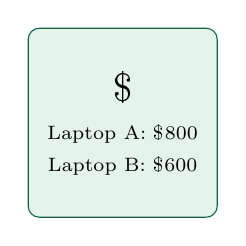
\begin{tikzpicture}
  \node[draw=ForestGreen,rounded corners,fill=SoftGreen,
        minimum width=2.4cm,minimum height=2.4cm] (box) {};

  \node[font=\Large] at ([yshift=0.45cm]box.center) {\$};
  \node[font=\scriptsize] at ([yshift=-0.15cm]box.center) {Laptop A: \$800};
  \node[font=\scriptsize] at ([yshift=-0.55cm]box.center) {Laptop B: \$600};
\end{tikzpicture}

\textbf{Online shopping}

\scriptsize
Sort by price or rating
\end{column}

% ------------------------------------------------
\begin{column}{0.23\textwidth}
\centering
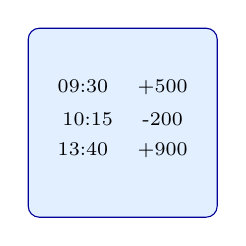
\begin{tikzpicture}
  \node[draw=blue!60!black,rounded corners,fill=SoftBlue,
        minimum width=2.4cm,minimum height=2.4cm] (box) {};

  \node[font=\scriptsize] at ([yshift=0.45cm]box.center) {09:30 \quad +500};
  \node[font=\scriptsize] at ([yshift=0.05cm]box.center) {10:15 \quad -200};
  \node[font=\scriptsize] at ([yshift=-0.35cm]box.center) {13:40 \quad +900};
\end{tikzpicture}

\textbf{Transactions}

\scriptsize
Sort by time or amount
\end{column}

% ------------------------------------------------
\begin{column}{0.23\textwidth}
\centering
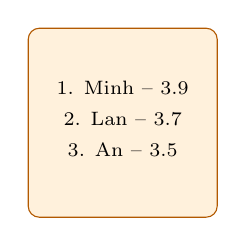
\begin{tikzpicture}
  \node[draw=orange!70!black,rounded corners,fill=SoftOrange,
        minimum width=2.4cm,minimum height=2.4cm] (box) {};

  \node[font=\scriptsize] at ([yshift=0.45cm]box.center) {1. Minh -- 3.9};
  \node[font=\scriptsize] at ([yshift=0.05cm]box.center) {2. Lan -- 3.7};
  \node[font=\scriptsize] at ([yshift=-0.35cm]box.center) {3. An -- 3.5};
\end{tikzpicture}

\textbf{Student ranking}

\scriptsize
Sort by GPA
\end{column}

% ------------------------------------------------
\begin{column}{0.23\textwidth}
\centering
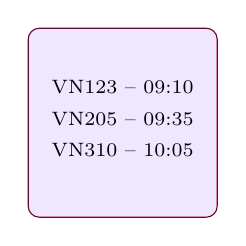
\begin{tikzpicture}
  \node[draw=purple!60!black,rounded corners,fill=SoftPurple,
        minimum width=2.4cm,minimum height=2.4cm] (box) {};

  \node[font=\scriptsize] at ([yshift=0.45cm]box.center) {VN123 -- 09:10};
  \node[font=\scriptsize] at ([yshift=0.05cm]box.center) {VN205 -- 09:35};
  \node[font=\scriptsize] at ([yshift=-0.35cm]box.center) {VN310 -- 10:05};
\end{tikzpicture}

\textbf{Flight schedule}

\scriptsize
Sort by departure time
\end{column}

\end{columns}

\vspace{0.6em}

\begin{alertblock}{What is common in all these examples?}
The same data becomes much easier to \textbf{compare, search, and use}
when it is placed in a meaningful order.
\end{alertblock}

\end{frame}

\begin{frame}{Why does sorting help?}
\small

\begin{columns}[T,onlytextwidth]

\begin{column}{0.45\textwidth}

\begin{block}{Unsorted data}
\[
[42,\;17,\;8,\;33,\;21,\;50,\;12]
\]

\vspace{0.4em}

\begin{center}
\textbf{Find 33}

\medskip

Where should we look first?
\end{center}

\end{block}

\end{column}

\begin{column}{0.08\textwidth}
\centering
\vspace{1.6cm}
\Huge$\Longrightarrow$
\end{column}

\begin{column}{0.45\textwidth}

\begin{exampleblock}{Sorted data}
\[
[8,\;12,\;17,\;21,\;33,\;42,\;50]
\]

\vspace{0.4em}

\begin{center}
\textbf{Find 33}

\medskip

Now the order gives us information.
\end{center}

\end{exampleblock}

\end{column}

\end{columns}

\vspace{0.35em}

\begin{alertblock}{Sorting is often not the final goal}
We usually sort data because the \textbf{next operation} becomes easier:
searching, ranking, detecting duplicates, finding extremes, or reporting.
\end{alertblock}

\end{frame}


\begin{frame}{What is sorting?}
\small

\begin{block}{Sorting}
Sorting rearranges a collection of records according to a specified
\textbf{key} and \textbf{order}.
\end{block}

\vspace{0.35em}

\begin{center}

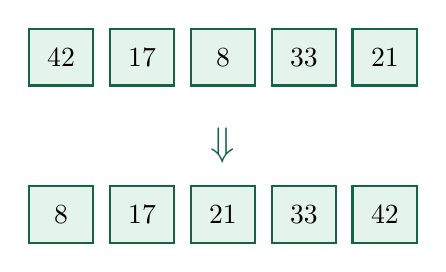
\begin{tikzpicture}[node distance=0.18cm]

\node[cell] (a1) {42};
\node[cell,right=of a1] (a2) {17};
\node[cell,right=of a2] (a3) {8};
\node[cell,right=of a3] (a4) {33};
\node[cell,right=of a4] (a5) {21};

\node[below=0.4cm of a3,font=\Large,ForestGreen] (arrow)
  {$\Downarrow$};

\node[cell,below=1.25cm of a1] (b1) {8};
\node[cell,right=of b1] (b2) {17};
\node[cell,right=of b2] (b3) {21};
\node[cell,right=of b3] (b4) {33};
\node[cell,right=of b4] (b5) {42};

\end{tikzpicture}

\end{center}

\vspace{0.25em}

\[
k(A[0])\leq k(A[1])\leq\cdots\leq k(A[n-1])
\]

\begin{alertblock}{But there is more than one way to create this order}
Different sorting algorithms use very different strategies.
\end{alertblock}

\end{frame}

\begin{frame}{The sorting problem must be specified precisely}
  \small
  \begin{block}{Problem specification}
    Given records $A[0..n-1]$ and a key function $k$, rearrange the records so
    that
    \[
      k(A[0])\le k(A[1])\le\cdots\le k(A[n-1]).
    \]
  \end{block}
  \begin{columns}[T]
    \begin{column}{0.48\textwidth}
      \begin{exampleblock}{Correctness requirements}
        \begin{itemize}
          \item The output is ordered by the chosen key.
          \item No input record is lost or duplicated.
        \end{itemize}
      \end{exampleblock}
    \end{column}
    \begin{column}{0.48\textwidth}
      \begin{alertblock}{Design questions}
        Is the sort stable? In-place? Adaptive? What are its best, average,
        and worst cases?
      \end{alertblock}
    \end{column}
  \end{columns}
\end{frame}

\begin{frame}{We already use sorting strategies in real life}
\footnotesize

\begin{columns}[T,onlytextwidth]

% ==========================================================
% INSERTION SORT
% ==========================================================
\begin{column}{0.235\textwidth}
\centering

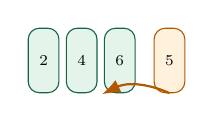
\begin{tikzpicture}[scale=0.78,transform shape]

% Cards
\foreach \x/\v in {0/2,0.62/4,1.24/6}{
  \node[
    draw=ForestGreen,
    fill=SoftGreen,
    rounded corners,
    minimum width=0.50cm,
    minimum height=1.05cm
  ] at (\x,0) {\scriptsize\v};
}

% New card
\node[
  draw=orange!70!black,
  fill=SoftOrange,
  rounded corners,
  minimum width=0.50cm,
  minimum height=1.05cm
] (new) at (2.05,0) {\scriptsize5};

\draw[
  -Latex,
  thick,
  orange!70!black
]
(new.south)
to[bend right=25]
(0.95,-0.55);

\end{tikzpicture}

\vspace{0.15em}

\textbf{Insertion Sort}

\vspace{0.1em}

\scriptsize
Insert a new card into an already sorted hand.

\end{column}


% ==========================================================
% BUBBLE SORT
% ==========================================================
\begin{column}{0.235\textwidth}
\centering

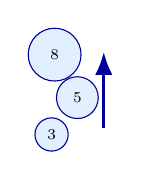
\begin{tikzpicture}[scale=0.78,transform shape]

\node[
  circle,
  draw=blue!60!black,
  fill=SoftBlue,
  minimum size=0.52cm
] at (0,-0.30) {\scriptsize3};

\node[
  circle,
  draw=blue!60!black,
  fill=SoftBlue,
  minimum size=0.68cm
] at (0.42,0.30) {\scriptsize5};

\node[
  circle,
  draw=blue!60!black,
  fill=SoftBlue,
  minimum size=0.86cm
] at (0.05,1.00) {\scriptsize8};

\draw[
  -Latex,
  very thick,
  blue!60!black
]
(0.85,-0.20) -- (0.85,1.05);

\end{tikzpicture}

\vspace{0.15em}

\textbf{Bubble Sort}

\vspace{0.1em}

\scriptsize
Large values gradually ``bubble'' toward the end.

\end{column}


% ==========================================================
% MERGE SORT
% ==========================================================
\begin{column}{0.235\textwidth}
\centering

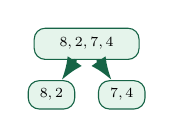
\begin{tikzpicture}[
  scale=0.72,
  transform shape
]

\node[
  draw=ForestGreen,
  fill=SoftGreen,
  rounded corners,
  minimum width=1.85cm,
  minimum height=0.55cm
] (all) at (0,0.75) {\scriptsize $8,2,7,4$};

\node[
  draw=ForestGreen,
  fill=SoftGreen,
  rounded corners,
  minimum width=0.82cm,
  minimum height=0.50cm
] (left) at (-0.62,-0.15) {\scriptsize $8,2$};

\node[
  draw=ForestGreen,
  fill=SoftGreen,
  rounded corners,
  minimum width=0.82cm,
  minimum height=0.50cm
] (right) at (0.62,-0.15) {\scriptsize $7,4$};

\draw[arrow] (all) -- (left);
\draw[arrow] (all) -- (right);

\end{tikzpicture}

\vspace{0.15em}

\textbf{Merge Sort}

\vspace{0.1em}

\scriptsize
Divide into smaller parts, sort them, then merge.

\end{column}


% ==========================================================
% QUICK SORT
% ==========================================================
\begin{column}{0.235\textwidth}
\centering

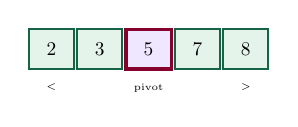
\begin{tikzpicture}[
  scale=0.70,
  transform shape,
  node distance=0.03cm
]

\node[cell] (q1) {2};
\node[cell,right=of q1] (q2) {3};
\node[pivot,right=of q2] (qp) {5};
\node[cell,right=of qp] (q3) {7};
\node[cell,right=of q3] (q4) {8};

\node[below=0.12cm of q1,font=\tiny] {$<$};
\node[below=0.12cm of qp,font=\tiny] {pivot};
\node[below=0.12cm of q4,font=\tiny] {$>$};

\end{tikzpicture}

\vspace{0.15em}

\textbf{Quick Sort}

\vspace{0.1em}

\scriptsize
Choose a pivot and split values into two groups.

\end{column}

\end{columns}

\vspace{0.35em}

\begin{alertblock}{The important question}
\centering
How does each strategy create order, and how much work does it require?
\end{alertblock}

\end{frame}

\begin{frame}{Vocabulary for comparing sorting algorithms}
  \small
  \begin{center}
    \begin{tabular}{L{0.18\textwidth}L{0.70\textwidth}}
      \toprule
      \textbf{Property} & \textbf{Meaning} \\
      \midrule
      Stable & Equal-key records keep their original relative order. \\
      In-place & Uses only a small amount of auxiliary memory. \\
      Adaptive & Runs faster when the input is already partly sorted. \\
      Comparison sort & Learns the order by comparing pairs of keys. \\
      Integer-key sort & Uses keys as array indices or digits, not only pairwise comparisons. \\
      Online & Can place new items as they arrive, without seeing all input. \\
      \bottomrule
    \end{tabular}
  \end{center}
  \begin{alertblock}{Running example}
    We will repeatedly sort $[7,3,5,2,6,4]$ and count comparisons, movements,
    recursion, and extra storage.
  \end{alertblock}
\end{frame}


% =============================================================
\section{Insertion Sort and Bubble Sort}
% =============================================================

\begin{frame}{Insertion sort: like arranging cards in your hand}
\small

\begin{columns}[T,onlytextwidth]

\begin{column}{0.52\textwidth}

\begin{center}
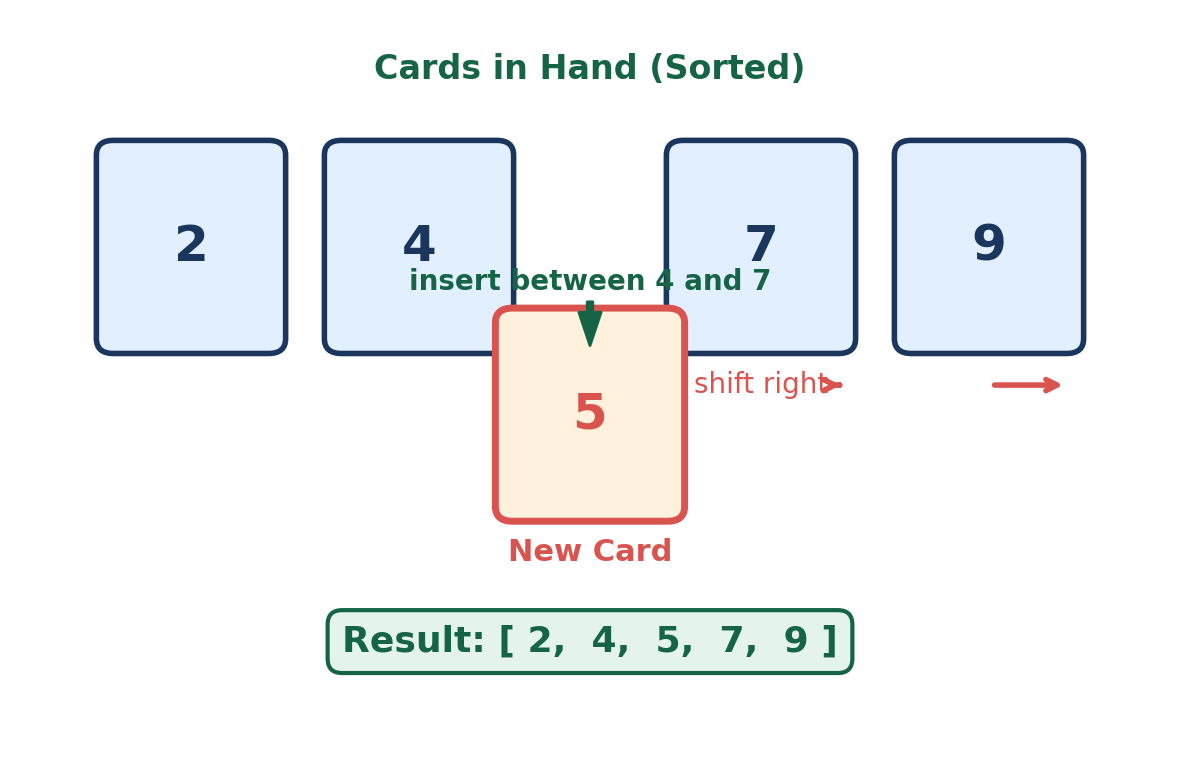
\includegraphics[width=0.94\linewidth]{insertion_page12_preview_v2/page12_insertion_arrow_top_preview_v2.png}
\end{center}

\end{column}

\begin{column}{0.44\textwidth}

\begin{block}{What would you do?}
You already hold
\[
2,\;4,\;7,\;9.
\]

A new card, $5$, arrives.
\end{block}

\begin{exampleblock}{Natural strategy}
\begin{enumerate}
\item Compare $5$ with the cards.
\item Move larger cards to the right.
\item Insert $5$ between $4$ and $7$.
\end{enumerate}
\end{exampleblock}

\end{column}

\end{columns}

\vspace{0.3em}

\centering
\Large
\textbf{That is the idea behind Insertion Sort.}

\end{frame}

\begin{frame}{Trace insertion sort}
  \small
  \begin{center}
    \renewcommand{\arraystretch}{1.25}
    \begin{tabular}{ccl}
      \toprule
      \textbf{Pass} & \textbf{Key} & \textbf{Sequence after insertion} \\
      \midrule
      Start & -- & $[7,3,5,2,6,4]$ \\
      1 & $3$ & $[3,7,5,2,6,4]$ \\
      2 & $5$ & $[3,5,7,2,6,4]$ \\
      3 & $2$ & $[2,3,5,7,6,4]$ \\
      4 & $6$ & $[2,3,5,6,7,4]$ \\
      5 & $4$ & $[2,3,4,5,6,7]$ \\
      \bottomrule
    \end{tabular}
  \end{center}
  \begin{alertblock}{Trace invariant}
    At the end of pass $i$, the prefix $A[0..i]$ is sorted and contains exactly
    the original records from that prefix.
  \end{alertblock}
\end{frame}

\begin{frame}[fragile]{Insertion-sort pseudocode}
  \begin{columns}[T]
    \begin{column}{0.56\textwidth}
\begin{lstlisting}[style=pseudonumbered]
FUNCTION INSERTION_SORT(A)
INPUT: array A of length n
OUTPUT: A sorted in non-decreasing order
    FOR i = 1 TO n - 1 DO
        key = A[i]
        j = i - 1
        WHILE j >= 0 AND A[j] > key DO
            A[j + 1] = A[j]
            j = j - 1
        A[j + 1] = key
    RETURN A
\end{lstlisting}
    \end{column}
    \begin{column}{0.40\textwidth}
      \begin{block}{What costs time?}
        Comparisons with \texttt{key} and shifts of larger elements.
      \end{block}
      \begin{exampleblock}{Why stable?}
        Equal items are not shifted past each other because the test uses
        \texttt{>} rather than \texttt{>=}.
      \end{exampleblock}
    \end{column}
  \end{columns}
\end{frame}

\begin{frame}{Insertion sort: correctness and complexity}
  \small
  \begin{columns}[T]
    \begin{column}{0.48\textwidth}
      \begin{block}{Correctness argument}
        \begin{enumerate}
          \item Before a pass, the prefix is sorted.
          \item Shifting opens the correct position for the key.
          \item Inserting the key preserves order and all records.
          \item After the final pass, the whole array is sorted.
        \end{enumerate}
      \end{block}
    \end{column}
    \begin{column}{0.48\textwidth}
      \begin{exampleblock}{Performance}
        \begin{itemize}
          \item Best case: $\Theta(n)$
          \item Average case: $\Theta(n^2)$
          \item Worst case: $\Theta(n^2)$
          \item Auxiliary space: $\Theta(1)$
        \end{itemize}
      \end{exampleblock}
      \begin{alertblock}{Best use}
        Small inputs or inputs that are already nearly sorted.
      \end{alertblock}
    \end{column}
  \end{columns}
\end{frame}

\begin{frame}{Activity: predict insertion-sort work}
  \begin{columns}[T]
    \begin{column}{0.48\textwidth}
      \begin{block}{Input A}
        $[1,2,3,4,5,6]$
      \end{block}
      \begin{exampleblock}{Input B}
        $[6,5,4,3,2,1]$
      \end{exampleblock}
    \end{column}
    \begin{column}{0.48\textwidth}
      \begin{alertblock}{Student task}
        For each input:
        \begin{enumerate}
          \item Count the successful shifts.
          \item Identify the best or worst case.
          \item Explain why the two inputs produce different work.
        \end{enumerate}
      \end{alertblock}
    \end{column}
  \end{columns}
\end{frame}

\begin{frame}{Why is it called Bubble Sort?}
\small

\begin{columns}[T,onlytextwidth]

\begin{column}{0.42\textwidth}

\begin{center}
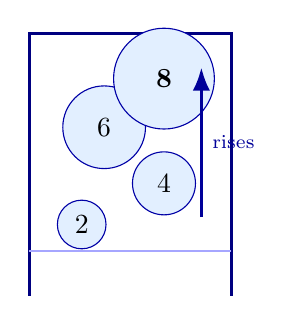
\begin{tikzpicture}[scale=0.95]

% water container
\draw[very thick,blue!50!black]
  (-1.35,-1.7) -- (-1.35,1.8)
  -- (1.35,1.8)
  -- (1.35,-1.7);

\draw[blue!35,thick]
  (-1.35,-1.1) -- (1.35,-1.1);

% bubbles
\node[circle,draw=blue!65!black,fill=SoftBlue,
      minimum size=0.60cm] at (-0.65,-0.75) {2};

\node[circle,draw=blue!65!black,fill=SoftBlue,
      minimum size=0.80cm] at (0.45,-0.20) {4};

\node[circle,draw=blue!65!black,fill=SoftBlue,
      minimum size=1.05cm] at (-0.35,0.55) {6};

\node[circle,draw=blue!65!black,fill=SoftBlue,
      minimum size=1.28cm] at (0.45,1.20) {\textbf{8}};

\draw[-Latex,very thick,blue!60!black]
  (0.95,-0.65) -- (0.95,1.35)
  node[midway,right,font=\scriptsize]{rises};

\end{tikzpicture}
\end{center}

\end{column}

\begin{column}{0.54\textwidth}

\begin{block}{Think about bubbles in water}
Larger bubbles rise toward the surface.
\end{block}

\begin{exampleblock}{Bubble Sort uses a similar visual idea}
Adjacent values are repeatedly compared.

If they are in the wrong order, they swap.

As comparisons continue, a large value moves step by step toward
the end of the array.
\end{exampleblock}

\begin{alertblock}{After one complete pass}
The largest remaining value has reached its final position.
\end{alertblock}

\end{column}

\end{columns}

\end{frame}

\begin{frame}{From the bubble idea to an array}
\small

\begin{center}

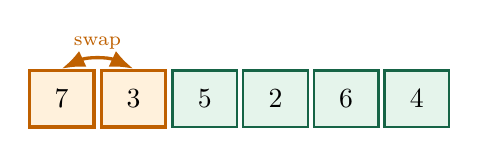
\begin{tikzpicture}[node distance=0.05cm]

\node[active] (a1) {7};
\node[active,right=of a1] (a2) {3};
\node[cell,right=of a2] (a3) {5};
\node[cell,right=of a3] (a4) {2};
\node[cell,right=of a4] (a5) {6};
\node[cell,right=of a5] (a6) {4};

\draw[<->,>=Latex,very thick,orange!75!black]
(a1.north) to[bend left=25]
node[above,font=\scriptsize]{swap}
(a2.north);

\end{tikzpicture}

\vspace{-0.2em}

\[
\renewcommand{\arraystretch}{1.05}
\begin{array}{c}
[7,3,5,2,6,4] \\[0.15em]
\Downarrow \\[0.15em]
[3,7,5,2,6,4] \\[0.15em]
\Downarrow \\[0.15em]
[3,5,7,2,6,4] \\[0.15em]
\Downarrow\ \cdots\ \Downarrow \\[0.15em]
[3,5,2,6,4,\boxed{7}]
\end{array}
\]

\end{center}

\vspace{-0.2em}

\begin{alertblock}{One pass}
The value $7$ does not jump directly to the end.
It moves there through a sequence of \textbf{adjacent comparisons and swaps}.
\end{alertblock}

\end{frame}

\begin{frame}{Bubble sort: repeatedly move the largest value right}
  \begin{block}{One pass}
    Compare adjacent values. Swap them when they are out of order. After one
    full pass, the largest remaining value reaches its final position.
  \end{block}
  \begin{center}
    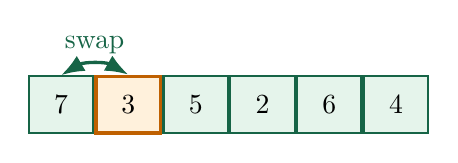
\begin{tikzpicture}[node distance=0pt]
      \node[cell] (a0) {7};
      \node[active,right=of a0] (a1) {3};
      \node[cell,right=of a1] (a2) {5};
      \node[cell,right=of a2] (a3) {2};
      \node[cell,right=of a3] (a4) {6};
      \node[cell,right=of a4] (a5) {4};
      \draw[<->,>=Latex,very thick,ForestGreen] (a0.north) to[bend left=30] node[above]{swap} (a1.north);
    \end{tikzpicture}
  \end{center}
  \begin{exampleblock}{After the first complete pass}
    $[3,5,2,6,4,7]$; the final $7$ never needs to move again.
  \end{exampleblock}
\end{frame}

\begin{frame}{Trace bubble sort by passes}
  \small
  \begin{center}
    \begin{tabular}{ccl}
      \toprule
      \textbf{Pass} & \textbf{Fixed suffix} & \textbf{Sequence after pass} \\
      \midrule
      Start & none & $[7,3,5,2,6,4]$ \\
      1 & $[7]$ & $[3,5,2,6,4,7]$ \\
      2 & $[6,7]$ & $[3,2,5,4,6,7]$ \\
      3 & $[5,6,7]$ & $[2,3,4,5,6,7]$ \\
      4 & no swaps & stop early \\
      \bottomrule
    \end{tabular}
  \end{center}
  \begin{alertblock}{Pass invariant}
    After each pass, the largest value in the unsorted prefix has moved to its
    final position.
  \end{alertblock}
\end{frame}

\begin{frame}[fragile]{Optimized bubble-sort pseudocode}
  \begin{columns}[T]
    \begin{column}{0.58\textwidth}
\begin{lstlisting}[style=pseudonumbered]
FUNCTION BUBBLE_SORT(A)
INPUT: array A of length n
OUTPUT: A sorted in non-decreasing order
    FOR end = LENGTH(A) - 1 DOWNTO 1 DO
        swapped = FALSE
        FOR i = 0 TO end - 1 DO
            IF A[i] > A[i + 1] THEN
                SWAP A[i], A[i + 1]
                swapped = TRUE
        IF swapped == FALSE THEN
            RETURN A
    RETURN A
\end{lstlisting}
    \end{column}
    \begin{column}{0.38\textwidth}
      \begin{block}{Performance}
        Best: $\Theta(n)$ with early stopping.\\
        Average/worst: $\Theta(n^2)$.\\
        Space: $\Theta(1)$.
      \end{block}
      \begin{alertblock}{Teaching value}
        Simple to visualize, but rarely the best general-purpose choice.
      \end{alertblock}
    \end{column}
  \end{columns}
\end{frame}

\begin{frame}{Activity: insertion sort or bubble sort?}
  \begin{columns}[T]
    \begin{column}{0.48\textwidth}
      \begin{block}{Input}
        $[1,2,3,5,4,6,7]$
      \end{block}
      \begin{exampleblock}{Work to record}
        Count comparisons, shifts, and swaps for both algorithms.
      \end{exampleblock}
    \end{column}
    \begin{column}{0.48\textwidth}
      \begin{alertblock}{Discussion}
        \begin{enumerate}
          \item Which algorithm moves fewer records?
          \item Where does early stopping help?
          \item Which invariant is easier to use when tracing?
        \end{enumerate}
      \end{alertblock}
    \end{column}
  \end{columns}
\end{frame}

% =============================================================
\section{Merge Sort and Quick Sort}
% =============================================================

\begin{frame}{Merge sort: merge two already sorted lines}
\footnotesize

\begin{columns}[T,onlytextwidth]

% ==========================================================
% LEFT: IDEA
% ==========================================================
\begin{column}{0.39\textwidth}

\textbf{Imagine two sorted queues}

\vspace{0.15em}

\[
A=[155,\;168,\;180]
\]

\vspace{-0.3em}

\[
B=[160,\;170,\;175]
\]

\vspace{0.15em}

\begin{exampleblock}{How do we merge them?}
Compare the \textbf{first remaining values}.

Move the smaller one to the output, then repeat.
\end{exampleblock}

\end{column}


% ==========================================================
% RIGHT: VISUALIZATION
% ==========================================================
\begin{column}{0.57\textwidth}

\centering

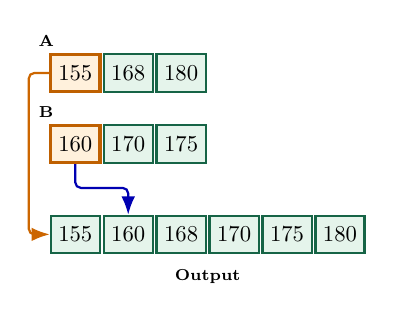
\begin{tikzpicture}[
  scale=0.82,
  transform shape,
  smallcell/.style={
    draw=ForestGreen,
    fill=SoftGreen,
    thick,
    minimum width=0.68cm,
    minimum height=0.58cm,
    align=center
  },
  firstcell/.style={
    draw=orange!75!black,
    fill=SoftOrange,
    very thick,
    minimum width=0.68cm,
    minimum height=0.58cm,
    align=center
  }
]

% Queue A
\node[font=\scriptsize\bfseries] at (-0.45,2.65) {A};
\node[firstcell] (a1) at (0,2.15) {155};
\node[smallcell] (a2) at (0.82,2.15) {168};
\node[smallcell] (a3) at (1.64,2.15) {180};

% Queue B
\node[font=\scriptsize\bfseries] at (-0.45,1.55) {B};
\node[firstcell] (b1) at (0,1.05) {160};
\node[smallcell] (b2) at (0.82,1.05) {170};
\node[smallcell] (b3) at (1.64,1.05) {175};

% Output row
\node[smallcell] (o1) at (0,-0.35) {155};
\node[smallcell] (o2) at (0.82,-0.35) {160};
\node[smallcell] (o3) at (1.64,-0.35) {168};
\node[smallcell] (o4) at (2.46,-0.35) {170};
\node[smallcell] (o5) at (3.28,-0.35) {175};
\node[smallcell] (o6) at (4.10,-0.35) {180};
\node[below=0.42cm of $(o3)!0.5!(o4)$,font=\scriptsize\bfseries] {Output};

% Arrows routed through whitespace only
\draw[-Latex,thick,orange!80!black,rounded corners=2pt]
  (a1.west) -- (-0.72,2.15) -- (-0.72,-0.35) -- (o1.west);

\draw[-Latex,thick,blue!70!black,rounded corners=2pt]
  (b1.south) -- (0,0.37) -- (0.82,0.37) -- (o2.north);

\end{tikzpicture}

\end{column}

\end{columns}

\vspace{0.25em}

\centering
\color{ForestGreen}
\textbf{Merge step: compare the two front values and repeatedly take the smaller one.}

\end{frame}

\begin{frame}{Merge sort: divide, solve, combine}
  \begin{center}
    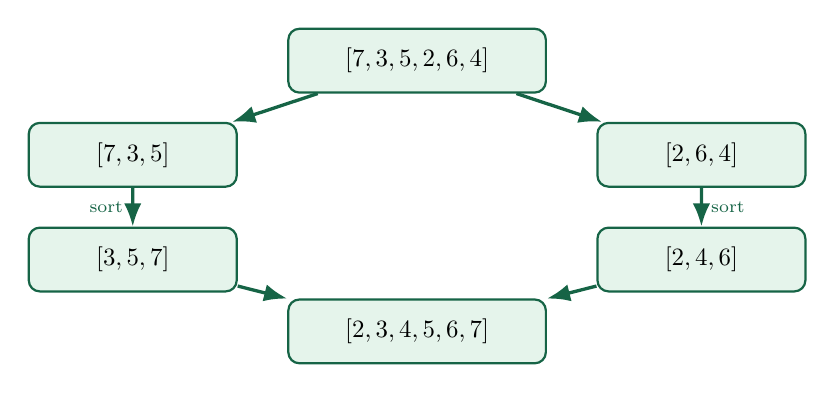
\begin{tikzpicture}[node distance=0.40cm and 0.70cm,scale=0.90,transform shape]
      \node[process,text width=3.4cm] (whole) {$[7,3,5,2,6,4]$};
      \node[process,below left=of whole] (left) {$[7,3,5]$};
      \node[process,below right=of whole] (right) {$[2,6,4]$};
      \node[process,below=0.55cm of left] (sl) {$[3,5,7]$};
      \node[process,below=0.55cm of right] (sr) {$[2,4,6]$};
      \node[process,text width=3.4cm,below=0.55cm of $(sl)!0.5!(sr)$] (out)
        {$[2,3,4,5,6,7]$};
      \draw[arrow] (whole) -- (left);
      \draw[arrow] (whole) -- (right);
      \draw[arrow] (left) -- node[left,font=\scriptsize]{sort} (sl);
      \draw[arrow] (right) -- node[right,font=\scriptsize]{sort} (sr);
      \draw[arrow] (sl) -- (out);
      \draw[arrow] (sr) -- (out);
    \end{tikzpicture}
  \end{center}
  \begin{alertblock}{Key insight}
    Merging two sorted sequences is linear; merge sort creates such sequences
    recursively.
  \end{alertblock}
\end{frame}

\begin{frame}{Trace the merge operation}
  \small
  \begin{block}{Merge $L=[3,5,7]$ and $R=[2,4,6]$}
    Compare only the first unmerged value in each sequence.
  \end{block}
  \begin{center}
    \begin{tabular}{ccl}
      \toprule
      \textbf{Compare} & \textbf{Take} & \textbf{Output so far} \\
      \midrule
      $3$ and $2$ & $2$ & $[2]$ \\
      $3$ and $4$ & $3$ & $[2,3]$ \\
      $5$ and $4$ & $4$ & $[2,3,4]$ \\
      $5$ and $6$ & $5$ & $[2,3,4,5]$ \\
      $7$ and $6$ & $6$ & $[2,3,4,5,6]$ \\
      right empty & $7$ & $[2,3,4,5,6,7]$ \\
      \bottomrule
    \end{tabular}
  \end{center}
\end{frame}

\begin{frame}[fragile]{Merge pseudocode}
  \begin{columns}[T]
    \begin{column}{0.62\textwidth}
\begin{lstlisting}[style=pseudonumbered]
FUNCTION MERGE(L, R)
INPUT: sorted lists L and R
OUTPUT: one sorted list containing all values
    result = empty list
    i = 0; j = 0
    WHILE i < LENGTH(L) AND j < LENGTH(R) DO
        IF L[i] <= R[j] THEN
            APPEND L[i] to result; i = i + 1
        ELSE
            APPEND R[j] to result; j = j + 1
    APPEND all remaining values of L
    APPEND all remaining values of R
    RETURN result
\end{lstlisting}
    \end{column}
    \begin{column}{0.34\textwidth}
      \begin{block}{Invariant}
        \texttt{result} is sorted and contains exactly the values already
        removed from $L$ and $R$.
      \end{block}
      \begin{alertblock}{Cost}
        At most $|L|+|R|-1$ key comparisons.
      \end{alertblock}
    \end{column}
  \end{columns}
\end{frame}

\begin{frame}[fragile]{Merge-sort pseudocode and recurrence}
  \begin{columns}[T]
    \begin{column}{0.55\textwidth}
\begin{lstlisting}[style=pseudonumbered]
FUNCTION MERGE_SORT(A)
INPUT: array A
OUTPUT: a sorted array containing the values of A
    IF LENGTH(A) <= 1 THEN
        RETURN A
    middle = LENGTH(A) DIV 2
    L = MERGE_SORT(A[0 : middle])
    R = MERGE_SORT(A[middle : end])
    RETURN MERGE(L, R)
\end{lstlisting}
    \end{column}
    \begin{column}{0.41\textwidth}
      \begin{block}{Running-time recurrence}
        \[
          T(n)=2T(n/2)+\Theta(n)
        \]
      \end{block}
      \begin{exampleblock}{Recursion tree}
        There are $\log_2 n$ levels, and each level performs $\Theta(n)$ merge
        work.
      \end{exampleblock}
      \centering
      $T(n)\in\Theta(n\log n)$
    \end{column}
  \end{columns}
\end{frame}

\begin{frame}{Merge sort: strengths and tradeoffs}
  \small
  \begin{columns}[T]
    \begin{column}{0.48\textwidth}
      \begin{exampleblock}{Strengths}
        \begin{itemize}
          \item $\Theta(n\log n)$ in every case
          \item Stable with a careful merge
          \item Natural for linked lists
          \item Useful for external sorting
        \end{itemize}
      \end{exampleblock}
    \end{column}
    \begin{column}{0.48\textwidth}
      \begin{alertblock}{Tradeoffs}
        \begin{itemize}
          \item Array implementation normally needs $\Theta(n)$ extra space
          \item Recursive calls add overhead
          \item Small subarrays may be faster with insertion sort
        \end{itemize}
      \end{alertblock}
    \end{column}
  \end{columns}
  \begin{block}{Hybrid idea}
    Practical implementations often use merge sort for large structure and
    insertion sort for small pieces.
  \end{block}
\end{frame}

\begin{frame}{Activity: perform one merge by hand}
  \begin{columns}[T]
    \begin{column}{0.48\textwidth}
      \begin{block}{Sorted inputs}
        \[
          L=[1,4,4,9],\qquad R=[2,4,7,8]
        \]
      \end{block}
      \begin{exampleblock}{Record while merging}
        Write the selected side, output sequence, and positions of the two
        front pointers after every comparison.
      \end{exampleblock}
    \end{column}
    \begin{column}{0.48\textwidth}
      \begin{alertblock}{Questions}
        \begin{enumerate}
          \item How many comparisons are made?
          \item Which $4$ is copied first?
          \item What condition makes the merge stable?
        \end{enumerate}
      \end{alertblock}
    \end{column}
  \end{columns}
\end{frame}

\begin{frame}{Quick Sort: choose a pivot and split the group}
\small

\begin{block}{Imagine organizing people by height}
Choose one person as the \textbf{pivot}.
Everyone shorter moves to one side;
everyone taller moves to the other side.
\end{block}

\vspace{0.4em}

\begin{center}

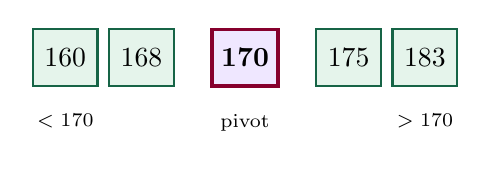
\begin{tikzpicture}[node distance=0.12cm]

\node[cell] (a1) {160};
\node[cell,right=of a1] (a2) {168};

\node[pivot,right=0.45cm of a2] (p) {\textbf{170}};

\node[cell,right=0.45cm of p] (a3) {175};
\node[cell,right=of a3] (a4) {183};

\node[below=0.22cm of a1,font=\scriptsize] {$<170$};
\node[below=0.22cm of p,font=\scriptsize] {pivot};
\node[below=0.22cm of a4,font=\scriptsize] {$>170$};

\end{tikzpicture}

\end{center}

\vspace{0.4em}

\begin{exampleblock}{Then repeat}
Sort the left group and the right group in exactly the same way.
\end{exampleblock}

\centering
\Large
\textbf{Partition first, then solve smaller problems.}

\end{frame}

\begin{frame}{Quicksort: partition around a pivot}
  \begin{block}{Partition goal}
    Rearrange the array so values smaller than the pivot are on its left and
    larger values are on its right. The pivot reaches its final sorted index.
  \end{block}
  \begin{center}
    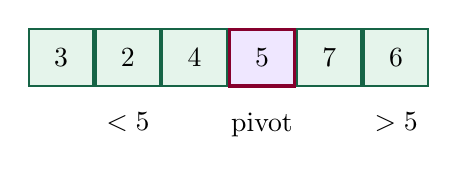
\begin{tikzpicture}[node distance=0pt]
      \node[cell] (a0) {3};
      \node[cell,right=of a0] (a1) {2};
      \node[cell,right=of a1] (a2) {4};
      \node[pivot,right=of a2] (a3) {5};
      \node[cell,right=of a3] (a4) {7};
      \node[cell,right=of a4] (a5) {6};
      \node[below=0.2cm of a1] {$<5$};
      \node[below=0.2cm of a3] {pivot};
      \node[below=0.2cm of a5] {$>5$};
    \end{tikzpicture}
  \end{center}
  \begin{alertblock}{Difference from merge sort}
    Quicksort performs the rearrangement before the recursive calls; merge sort
    combines results after them.
  \end{alertblock}
\end{frame}

\begin{frame}{Trace one partition}
  \small
  \begin{block}{Input $[7,3,5,2,6,4]$, choose pivot $4$}
    Scan the remaining values and maintain a boundary between values at most
    the pivot and values greater than it.
  \end{block}
  \begin{center}
    \begin{tabular}{ccl}
      \toprule
      \textbf{Scanned value} & \textbf{Action} & \textbf{Array state} \\
      \midrule
      $7$ & leave right & $[7,3,5,2,6,4]$ \\
      $3$ & move left & $[3,7,5,2,6,4]$ \\
      $5$ & leave right & $[3,7,5,2,6,4]$ \\
      $2$ & move left & $[3,2,5,7,6,4]$ \\
      $6$ & leave right & $[3,2,5,7,6,4]$ \\
      finish & place pivot & $[3,2,4,7,6,5]$ \\
      \bottomrule
    \end{tabular}
  \end{center}
\end{frame}

\begin{frame}[fragile]{Quicksort pseudocode}
  \begin{columns}[T]
    \begin{column}{0.58\textwidth}
\begin{lstlisting}[style=pseudo]
FUNCTION QUICK_SORT(A, low, high)
    IF low >= high THEN RETURN
    p = PARTITION(A, low, high)
    QUICK_SORT(A, low, p - 1)
    QUICK_SORT(A, p + 1, high)

FUNCTION PARTITION(A, low, high)
    pivot = A[high]
    boundary = low
    FOR scan = low TO high - 1 DO
        IF A[scan] <= pivot THEN
            SWAP A[boundary], A[scan]
            boundary = boundary + 1
    SWAP A[boundary], A[high]
    RETURN boundary
\end{lstlisting}
    \end{column}
    \begin{column}{0.38\textwidth}
      \begin{exampleblock}{Average behavior}
        Balanced partitions create about $\log n$ levels with $\Theta(n)$ work
        per level.
      \end{exampleblock}
      \begin{alertblock}{Worst behavior}
        Repeated splits of sizes $0$ and $n-1$ produce $\Theta(n^2)$ time.
      \end{alertblock}
    \end{column}
  \end{columns}
\end{frame}

\begin{frame}{Quicksort depends on pivot quality}
  \small
  \begin{columns}[T]
    \begin{column}{0.48\textwidth}
      \begin{block}{Complexity}
        \begin{itemize}
          \item Best/average: $\Theta(n\log n)$
          \item Worst: $\Theta(n^2)$
          \item Expected stack: $\Theta(\log n)$
          \item Worst stack: $\Theta(n)$
        \end{itemize}
      \end{block}
    \end{column}
    \begin{column}{0.48\textwidth}
      \begin{exampleblock}{Pivot strategies}
        \begin{itemize}
          \item Random pivot
          \item Median of first, middle, last
          \item Three-way partition for many duplicates
        \end{itemize}
      \end{exampleblock}
    \end{column}
  \end{columns}
  \begin{alertblock}{Practical strength}
    Good cache behavior and low constant factors make carefully implemented
    quicksort very fast for arrays.
  \end{alertblock}
\end{frame}

\begin{frame}{Activity: pivot choice changes the recursion}
  \small
  \begin{block}{Input}
    $[1,2,3,4,5,6,7,8]$
  \end{block}
  \begin{columns}[T]
    \begin{column}{0.48\textwidth}
      \begin{exampleblock}{Case A: last value as pivot}
        Sketch the partition sizes and recursion depth. Count the first three
        partition sizes.
      \end{exampleblock}
    \end{column}
    \begin{column}{0.48\textwidth}
      \begin{alertblock}{Case B: middle value as pivot}
        Sketch the partition tree and compare its height with Case A.
      \end{alertblock}
    \end{column}
  \end{columns}
  \begin{block}{Extension}
    Repeat with $[4,2,4,1,4,3,4]$. Why can a three-way partition help?
  \end{block}
\end{frame}


% =============================================================
\section{Counting Sort and Radix Sort}
% =============================================================

\begin{frame}{Beyond comparison sorting}
\small
\begin{columns}[T,onlytextwidth]
  \begin{column}{0.48\textwidth}
    \begin{block}{Comparison sorts}
      Insertion sort, bubble sort, merge sort, and quicksort learn the order by
      comparing two keys at a time.
      \[
        \text{``Is } A[i] \le A[j]\text{?''}
      \]
    \end{block}
    \begin{alertblock}{Lower-bound reminder}
      Any comparison-based sorting algorithm needs $\Omega(n\log n)$
      comparisons in the worst case.
    \end{alertblock}
  \end{column}
  \begin{column}{0.48\textwidth}
    \begin{exampleblock}{When keys are restricted}
      If keys are small integers, digits, or symbols from a known alphabet, we
      can use their values directly.
    \end{exampleblock}
    \begin{block}{Non-comparison idea}
      Count how many keys occur, or sort by one digit at a time using a stable
      subroutine.
    \end{block}
  \end{column}
\end{columns}
\vspace{0.3em}
\centering
\Large\color{ForestGreen}\textbf{Counting Sort and Radix Sort exploit structure in the keys.}
\end{frame}

\begin{frame}{Counting sort: count keys, then place items}
\small
\begin{columns}[T,onlytextwidth]
  \begin{column}{0.50\textwidth}
    \begin{block}{Assumption}
      Each key is an integer in a small known range:
      \[
        0 \le A[i] \le k.
      \]
    \end{block}
    \begin{exampleblock}{Core idea}
      \begin{enumerate}\setlength{\itemsep}{0.15em}
        \item Count occurrences of each key.
        \item Convert counts into positions using prefix sums.
        \item Place records into the output array in stable order.
      \end{enumerate}
    \end{exampleblock}
  \end{column}
  \begin{column}{0.48\textwidth}
    \centering
    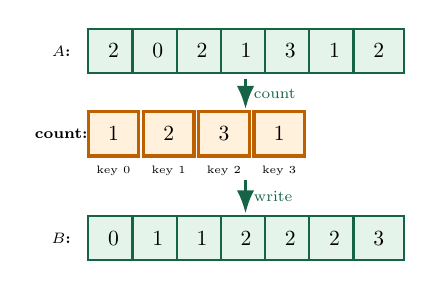
\begin{tikzpicture}[scale=0.78,transform shape]
      \node[font=\scriptsize\bfseries] at (-0.85,2.9) {$A$:};
      \foreach \i/\v in {0/2,1/0,2/2,3/1,4/3,5/1,6/2}{
        \node[cell] (a\i) at (\i*0.72,2.9) {\v};
      }
      \node[font=\scriptsize\bfseries] at (-0.85,1.55) {count:};
      \foreach \i/\v in {0/1,1/2,2/3,3/1}{
        \node[active] at (\i*0.9,1.55) {\v};
        \node[font=\tiny] at (\i*0.9,0.95) {key \i};
      }
      \node[font=\scriptsize\bfseries] at (-0.85,-0.15) {$B$:};
      \foreach \i/\v in {0/0,1/1,2/1,3/2,4/2,5/2,6/3}{
        \node[cell] at (\i*0.72,-0.15) {\v};
      }
      \draw[arrow] (2.15,2.45) -- node[right,font=\scriptsize]{count} (2.15,1.95);
      \draw[arrow] (2.15,0.80) -- node[right,font=\scriptsize]{write} (2.15,0.25);
    \end{tikzpicture}
  \end{column}
\end{columns}
\end{frame}

\begin{frame}[fragile]{Counting-sort pseudocode: stable version}
\scriptsize
\begin{columns}[T,onlytextwidth]
  \begin{column}{0.63\textwidth}
\begin{lstlisting}[style=pseudonumbered,basicstyle=\ttfamily\scriptsize]
FUNCTION COUNTING_SORT(A, k)
INPUT: array A of n integer keys in {0,...,k}
OUTPUT: stable sorted array B
    CREATE count[0..k] initialized to 0
    FOR i = 0 TO n - 1 DO
        count[A[i]] = count[A[i]] + 1
    FOR key = 1 TO k DO
        count[key] = count[key] + count[key - 1]
    CREATE output array B of length n
    FOR i = n - 1 DOWNTO 0 DO
        key = A[i]
        B[count[key] - 1] = A[i]
        count[key] = count[key] - 1
    RETURN B
\end{lstlisting}
  \end{column}
  \begin{column}{0.34\textwidth}
    \begin{block}{Why scan from right to left?}
      It preserves the relative order of equal keys, so the algorithm is
      \textbf{stable}.
    \end{block}
    \begin{exampleblock}{Complexity}
      \[
      \begin{aligned}
        T(n,k) &= \Theta(n+k),\\
        S(n,k) &= \Theta(n+k).
      \end{aligned}
      \]
    \end{exampleblock}
  \end{column}
\end{columns}
\end{frame}

\begin{frame}{Counting sort: when is it useful?}
\small
\begin{columns}[T,onlytextwidth]
  \begin{column}{0.48\textwidth}
    \begin{exampleblock}{Good situations}
      \begin{itemize}\setlength{\itemsep}{0.2em}
        \item Scores from $0$ to $100$.
        \item Ages, ratings, categories, small integer IDs.
        \item A stable subroutine inside radix sort.
      \end{itemize}
    \end{exampleblock}
  \end{column}
  \begin{column}{0.48\textwidth}
    \begin{alertblock}{Limitations}
      \begin{itemize}\setlength{\itemsep}{0.2em}
        \item Requires integer keys or mapped categories.
        \item Inefficient if $k$ is much larger than $n$.
        \item Usually not in-place because it uses an output array.
      \end{itemize}
    \end{alertblock}
  \end{column}
\end{columns}
\vspace{0.4em}
\begin{block}{Rule of thumb}
  Counting sort is attractive when $k=O(n)$, because then
  $\Theta(n+k)=\Theta(n)$.
\end{block}
\end{frame}

\begin{frame}{Radix sort: sort by digits}
\small
\begin{columns}[T,onlytextwidth]
  \begin{column}{0.42\textwidth}
    \begin{block}{Input idea}
      Suppose keys have $d$ digits in base $b$.
      \[
        329,\;457,\;657,\;839,\;436,\;720,\;355
      \]
    \end{block}
    \begin{exampleblock}{Least-significant-digit strategy}
      \begin{enumerate}\setlength{\itemsep}{0.15em}
        \item Stable sort by ones digit.
        \item Stable sort by tens digit.
        \item Stable sort by hundreds digit.
      \end{enumerate}
    \end{exampleblock}
  \end{column}
  \begin{column}{0.56\textwidth}
    \centering
    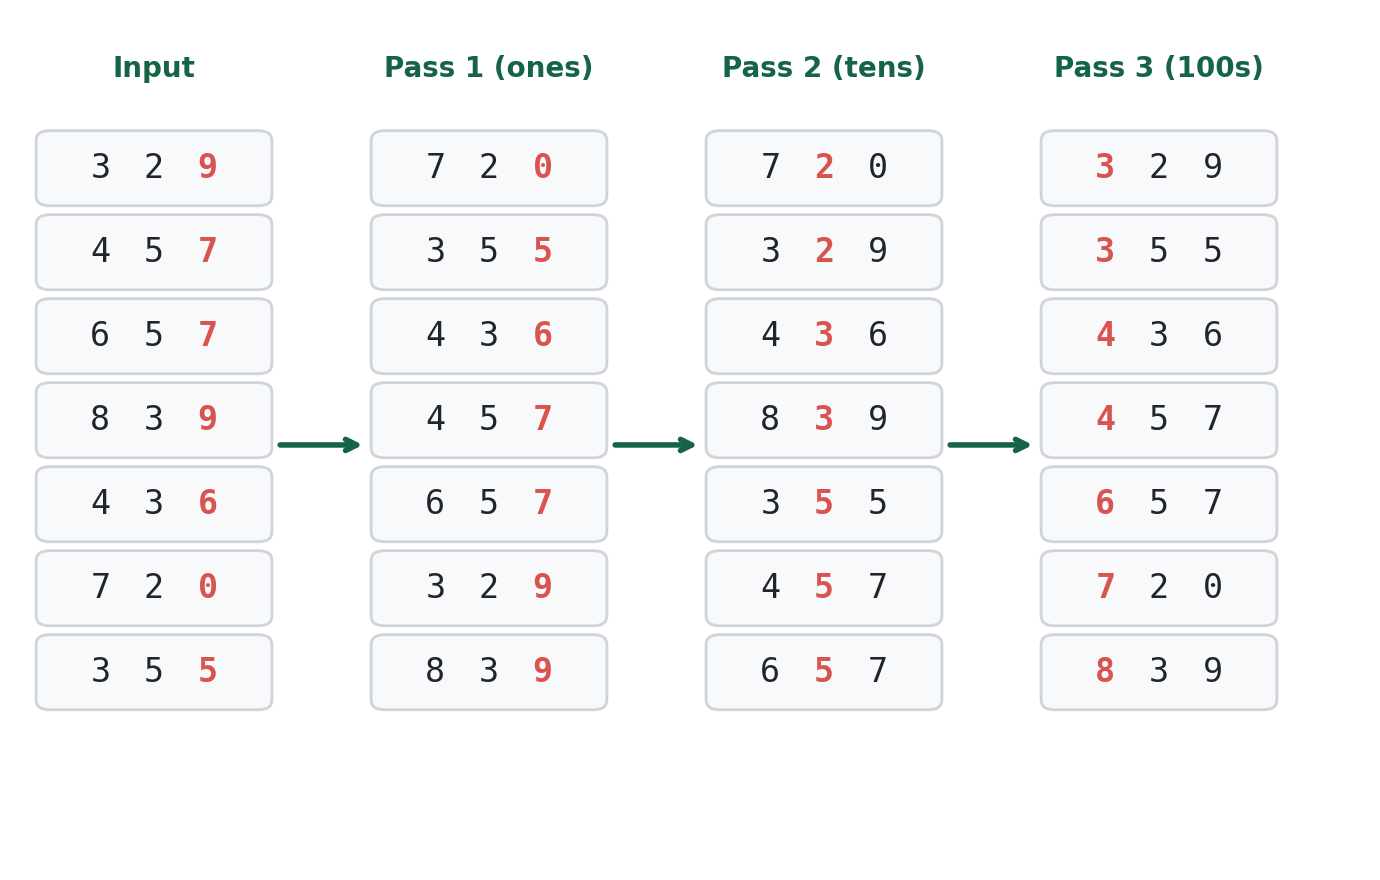
\includegraphics[width=0.99\linewidth]{radix_figure_assets_v4/page42_flow_only_v1.png}
  \end{column}
\end{columns}
\vspace{0.2em}
\begin{alertblock}{Why stability matters}
  When sorting by the next digit, equal digits must keep the order already
  established by less significant digits.
\end{alertblock}
\end{frame}

\begin{frame}[fragile]{Radix-sort pseudocode}
\scriptsize
\begin{columns}[T,onlytextwidth]
  \begin{column}{0.60\textwidth}
\begin{lstlisting}[style=pseudonumbered,basicstyle=\ttfamily\scriptsize]
FUNCTION RADIX_SORT(A, d, b)
INPUT: array A of n non-negative integer keys
OUTPUT: A sorted in non-decreasing order
    FOR digit_position = 0 TO d - 1 DO
        A = STABLE_COUNTING_SORT_BY_DIGIT(A,
            digit_position, b)
    RETURN A
\end{lstlisting}
  \end{column}
  \begin{column}{0.36\textwidth}
    \begin{block}{Cost per digit}
      Stable counting sort by one digit costs $\Theta(n+b)$.
    \end{block}
    \begin{exampleblock}{Total cost}
      \[
        T(n,d,b)=\Theta(d(n+b)).
      \]
      If $d$ and $b$ are treated as constants, this is linear in $n$.
    \end{exampleblock}
  \end{column}
\end{columns}
\end{frame}

\begin{frame}{Counting sort versus Radix sort}
\scriptsize
\begin{center}
\renewcommand{\arraystretch}{1.18}
\begin{tabular}{L{0.20\textwidth}L{0.33\textwidth}L{0.33\textwidth}}
\toprule
\textbf{Aspect} & \textbf{Counting Sort} & \textbf{Radix Sort} \\
\midrule
Key assumption & Keys are integers in $0..k$ & Keys have $d$ digits in base $b$ \\
Main idea & Count occurrences and compute positions & Stable-sort by one digit at a time \\
Stability & Stable if output is filled carefully & Requires a stable digit-sorting subroutine \\
Time & $\Theta(n+k)$ & $\Theta(d(n+b))$ \\
Extra space & $\Theta(n+k)$ & Usually $\Theta(n+b)$ per pass \\
Best when & Range $k$ is small & Fixed-length integer/string keys \\
\bottomrule
\end{tabular}
\end{center}
\begin{alertblock}{Common mistake}
  These algorithms are better only when their assumptions about the key domain are valid.
\end{alertblock}
\end{frame}

\begin{frame}{Activity: trace counting sort and radix sort}
\small
\begin{columns}[T,onlytextwidth]
  \begin{column}{0.48\textwidth}
    \begin{block}{Counting-sort task}
      Sort
      \[
        A=[2,0,2,1,3,1,2]
      \]
      with keys in $0..3$.
      \begin{enumerate}\setlength{\itemsep}{0.1em}
        \item Build the count array.
        \item Compute prefix sums.
        \item Fill the output array from right to left.
      \end{enumerate}
    \end{block}
  \end{column}
  \begin{column}{0.48\textwidth}
    \begin{exampleblock}{Radix-sort task}
      Sort
      \[
        [329,457,657,839,436,720,355]
      \]
      using LSD radix sort.
      \begin{enumerate}\setlength{\itemsep}{0.1em}
        \item Sort by ones digit.
        \item Sort by tens digit.
        \item Sort by hundreds digit.
      \end{enumerate}
    \end{exampleblock}
  \end{column}
\end{columns}
\end{frame}

% =============================================================
\section{Comparing Sorting Algorithms}
% =============================================================

\begin{frame}{Comparison of sorting algorithms}
  \scriptsize
  \begin{center}
    \begin{tabular}{L{0.16\textwidth}ccccL{0.24\textwidth}}
      \toprule
      \textbf{Algorithm} & \textbf{Best} & \textbf{Average} & \textbf{Worst} &
      \textbf{Extra space} & \textbf{Important property} \\
      \midrule
      Insertion & $n$ & $n^2$ & $n^2$ & $1$ & Stable, adaptive, excellent for small/nearly sorted data \\
      Bubble & $n$ & $n^2$ & $n^2$ & $1$ & Stable and simple, but performs many comparisons \\
      Merge & $n\log n$ & $n\log n$ & $n\log n$ & $n$ & Stable and predictable \\
      Quick & $n\log n$ & $n\log n$ & $n^2$ & $\log n$ expected & Usually fast in-place; normally unstable \\
      Counting & $n+k$ & $n+k$ & $n+k$ & $n+k$ & Linear when integer range $k$ is small \\
      Radix & $d(n+b)$ & $d(n+b)$ & $d(n+b)$ & $n+b$ & Sorts fixed-length keys by stable digit passes \\
      \bottomrule
    \end{tabular}
  \end{center}
  \begin{alertblock}{Do not choose from Big-$O$ alone}
    Input size, existing order, memory, record movement, stability, and worst-case
    guarantees can change the best choice.
  \end{alertblock}
\end{frame}

\begin{frame}{Choose an algorithm for the situation}
  \begin{columns}[T]
    \begin{column}{0.48\textwidth}
      \begin{block}{Scenarios}
        \begin{enumerate}
          \item Twenty nearly sorted records
          \item Millions of records with a stability requirement
          \item Large in-memory numeric array
          \item Scores in the range $0..100$
          \item Fixed-length student ID numbers
          \item Data larger than available RAM
        \end{enumerate}
      \end{block}
    \end{column}
    \begin{column}{0.48\textwidth}
      \begin{exampleblock}{Likely choices}
        \begin{enumerate}
          \item Insertion sort
          \item Merge-based stable sort
          \item Carefully implemented quicksort or a library sort
          \item Counting sort
          \item Radix sort
          \item External merge sort
        \end{enumerate}
      \end{exampleblock}
    \end{column}
  \end{columns}
  \begin{alertblock}{Discussion}
    Which additional facts could change each decision?
  \end{alertblock}
\end{frame}

% =============================================================
\section{Python's Built-In Sorting Functions}
% =============================================================

\begin{frame}[fragile]{\texttt{sorted()} versus \texttt{list.sort()}}
  \begin{columns}[T]
    \begin{column}{0.49\textwidth}
      \begin{block}{\texttt{sorted(iterable)}}
\begin{lstlisting}[language=Python,basicstyle=\ttfamily\scriptsize]
values = [7, 3, 5, 2]
result = sorted(values)
# values is unchanged
# result is [2, 3, 5, 7]
\end{lstlisting}
        Returns a new list and accepts any iterable.
      \end{block}
    \end{column}
    \begin{column}{0.49\textwidth}
      \begin{exampleblock}{\texttt{list.sort()}}
\begin{lstlisting}[language=Python,basicstyle=\ttfamily\scriptsize]
values = [7, 3, 5, 2]
answer = values.sort()
# values is now sorted
# answer is None
\end{lstlisting}
        Modifies the list in place and returns \texttt{None}.
      \end{exampleblock}
    \end{column}
  \end{columns}
\end{frame}

\begin{frame}[fragile]{Sort records with \texttt{key} and \texttt{reverse}}
  \begin{lstlisting}[language=Python,basicstyle=\ttfamily\scriptsize]
students = [
    {"id": "S1", "name": "Lan", "gpa": 3.4},
    {"id": "S2", "name": "Minh", "gpa": 3.8},
    {"id": "S3", "name": "An", "gpa": 3.8},
]

ranked = sorted(students,
                key=lambda s: (-s["gpa"], s["name"]))
  \end{lstlisting}
  \begin{columns}[T]
    \begin{column}{0.48\textwidth}
      \begin{block}{Key function}
        Converts each record into the value or tuple used for comparison.
      \end{block}
    \end{column}
    \begin{column}{0.48\textwidth}
      \begin{exampleblock}{Python guarantee}
        Python sorting is stable, so equal-key records retain their previous
        relative order.
      \end{exampleblock}
    \end{column}
  \end{columns}
\end{frame}

\begin{frame}{Common sorting mistakes}
  \begin{columns}[T]
    \begin{column}{0.48\textwidth}
      \begin{alertblock}{Mistakes}
        \begin{itemize}
          \item Expecting \texttt{list.sort()} to return the list
          \item Sorting numbers stored as strings
          \item Writing a comparison key with inconsistent types
          \item Forgetting whether the original list may be modified
        \end{itemize}
      \end{alertblock}
    \end{column}
    \begin{column}{0.48\textwidth}
      \begin{exampleblock}{Good workflow}
        \begin{enumerate}
          \item Define the required order precisely.
          \item Choose the key and direction.
          \item Decide whether a copy is needed.
          \item Test duplicates and boundary cases.
        \end{enumerate}
      \end{exampleblock}
    \end{column}
  \end{columns}
\end{frame}

\begin{frame}[fragile]{Integrated activity: sort transaction records}
  \begin{block}{Task}
    Sort transactions by date ascending; for equal dates, sort amount
    descending; preserve input order when both keys are equal.
  \end{block}
\begin{lstlisting}[language=Python,basicstyle=\ttfamily\scriptsize]
transactions = [
    {"date": "2026-08-10", "amount": 250, "id": "T1"},
    {"date": "2026-08-09", "amount": 400, "id": "T2"},
    {"date": "2026-08-10", "amount": 300, "id": "T3"},
    {"date": "2026-08-10", "amount": 250, "id": "T4"},
]
\end{lstlisting}
  \begin{alertblock}{Student questions}
    Write the key function, predict the output IDs, and explain where stability
    matters.
  \end{alertblock}
\end{frame}

\begin{frame}{Key takeaways}
  \begin{itemize}
    \item Sorting requires both an ordering rule and preservation of all records.
    \item Insertion sort is adaptive and effective for small or nearly sorted input.
    \item Merge sort guarantees $\Theta(n\log n)$ time and is naturally stable.
    \item Bubble sort is easy to understand but inefficient for general use.
    \item Quicksort is usually fast, but poor pivots can cause quadratic time.
    \item Counting sort and radix sort can be linear when keys have restricted structure.
    \item Python's stable built-in sort should be the default in application code;
      studying algorithms explains its tradeoffs and behavior.
  \end{itemize}
\end{frame}

\begin{frame}{After-class practice}
  \begin{enumerate}
    \item Trace all four algorithms on $[5,1,4,2,8,2]$.
    \item Count insertion-sort shifts for sorted and reverse-sorted arrays.
    \item Modify merge sort to order records by a supplied key function.
    \item Show an input that makes last-element-pivot quicksort quadratic.
    \item Trace counting sort on $[2,0,2,1,3,1,2]$.
    \item Trace one LSD radix-sort pass for three-digit numbers.
    \item Use Python to sort student records by class, descending GPA, and name.
  \end{enumerate}
\end{frame}

\end{document}